\section{Auswertung}
\label{sec:Auswertung}

\subsection{Die Aktivit"at der Americum-Quelle}
  Die Aktivit"at/Z"ahlrate $Z_{Quelle}$ der $^{241}\text{Am}$-Quelle wird gegeben druch
  \begin{equation}
    \frac{4\pi(\SI{0,041}{\meter}+\SI{0,039}{\meter}+\SI{0.017}{\meter})^2}{3F}Z_{gemessen}
  \end{equation}
  ,weil davon ausgegangen wird, dass die Quelle homogen in alle Raumrichtungen strahlt.
  Mit $Z_{gemessen}=\SI{13,5}{\becquerel}$ ergibt sich:
  \begin{equation}
    Z_{Quelle} = \SI{274}{\kilo \becquerel} \; .
  \end{equation}

  Der theoretisch zu erwartende Wert kann mithilfe des klassischen Zerfallsgesetzes berechnet werden:
  \begin{equation}
    Z_{Quelle} = Z_0\text{e}^{\frac{\ln(2)t}{\tau}} \approx \SI{318}{\kilo \becquerel}
  \end{equation}
  Dabei ist $\tau=432,2$ Jahre die Halbwertszeit und $Z_0=\SI{330}{\kilo \becquerel}$ \cite{Anleitung} die urspr"ungliche Aktivit"at.


\subsection{\texorpdfstring{Bestimmung der Foliendicke einer Goldfolie durch Energieverlustmessung der $\alpha$-Teilchen}{Bestimmung der Foliendicke einer Goldfolie durch Energieverlustmessung der alpha-Teilchen}}
Um die Foliendicke zu bestimmen wurde eine Energieverlustmessung durchgeführt. Die Messwerte sind in Tabelle \ref{tab:mit} und \ref{tab:ohne} aufgetragen. 
\begin{table}[H] 
	\centering
	\begin{tabular}{c|c}

		Druck  [mbar]& Pulshöhe [mV] \\ 
		\hline 
0,059	&1020 \\
20	&960 \\
30	&900\\
40	&860\\
50	&840\\
60	&820\\
70	&720\\
80	&740\\
90	&730\\
100	&680\\
110	&640\\
120	&620\\
130	&610\\
140	&600\\	
		
	\end{tabular} 
	\caption{Messwerte für die Energieverlustmessung mit Folie } 
	  \label{tab:mit}
\end{table}  

\begin{table}[H] 
	\centering
	\begin{tabular}{c|c}

	Druck[mbar] & Pulshöhe  [V] \\ 
		\hline 
0,07	& 1480\\
40	& 1300\\
80	& 1160\\
120	& 1040\\
140	& 940\\
	
	\end{tabular} 
	\caption{Messwerte für die Energieverlustmessung ohne Folie } 
	\label{tab:ohne}
\end{table} 

Die Werte für die Pulshöhe werden gegen den Druck aufgetragen. Eine lineare Funktion die durch $f(x)=a\cdot x+b$ gegeben ist wird an die Messwerte angepasst.
\begin{figure}[h]
	\centering
	\includegraphics[width=12cm,height=8cm]{auswertung/v16_plot1.pdf}
	\caption{Energieverlustmessung mit und ohne Goldfolie}
	\label{img:grafik-dummy}
\end{figure}
\newpage 
Aus der Ausgleichsrechnung ergeben sich für die Parameter a und b der Funktion $f(x)=a\cdot x+b$ für die Messung mit und ohne Goldfolie folgende Werte: 
\begin{align*}
a_{ohne}= -3,71 \pm 0,1602 \; \frac{1}{\text{mbar}}
\\
a_{mit}= -3,09 \pm 0,1578 \; \frac{1}{\text{mbar}}
\\
\\
b_{ohne}= 1466,4 \pm 14,68 \; \text{mV}
\\
b_{mit}= 996,82 \pm  13,43 \; \text{mV}
\end{align*}
Die Differenz dieser beiden Geraden entspricht dem Energieverlust durch die Folie. Die Differenz der Impulshöhen wird durch die Subtraktion der Achsenabschnitte bestimmt: 
\begin{align}
b_{ohne}-b_{mit}= 469,58 \pm 28,11 \; \text{mV}
\end{align} 
Um aus der Differenz der Impulshöhen einen Energiedifferenz zu erhalten wird die Impulshöhe beim Druck $p=0$ bei der Messung ohne Goldfolie der ursprünglichen Energie $E_\alpha$ zu geordnet. 

\begin{align*}
\Delta E= 1,7568 \pm 0,10\;  \text{MeV}  
\end{align*} 

Die Dicke der Folie $x$ wird mit dem Energieverlust und durch Umstellen der Bethe-Bloch-Gleichung (1) bestimmt. Dabei werden folgende materialabhängigen Parameter benutzt. Die Masse des $\alpha$-Teilchens lässt sich über $m=A \cdot u$ bestimmen. A ist die elementspezifische Massenzahl und u die atomare Masseneinheit. Für ein $\alpha$-Teilchen gilt A=4, sodass sich für die Masse folgender Wert ergibt: 

\begin{align*}
m_{\alpha}= 6.64 \cdot 10^{-27} \text{kg} 
\end{align*} 
Die Geschwindigkeit lässt sich damit mit der Formel 
\begin{align*}
v_{\alpha}= \sqrt{\frac{2\cdot E_{\alpha}}{m_{\alpha}}} 
\end{align*} 
bestimmen:
\begin{align*}
v_{\alpha}=16.27 \cdot 10^{6} \frac{\text{m}}{\text{s}}
\end{align*} 

Die Anzahl der Teilchen pro Volumeneinheit N lässt sich über \begin{align}
N= \frac{\rho}{m_{Atom}} 
\end{align} mit der Atommasse $m_{Atom}=A \cdot u$ bestimmen. 
Für die Dichte des Targetmaterials $\rho$ wird 19320 $\frac{\text{kg}}{\text{m}^3}$ $[1]$ eingesetzt. Daraus ergibt sich für die Masse von Gold 
 \begin{align*}
 N=5.91 \cdot 10^{28} \frac{1}{\text{m}^3}
 \end{align*} 
 Aus den berechneten Werten und der Ionisationsenergie von Gold $I=9.225 \frac{\text{eV}}{\text{atom}} \; [5]$ und den Ordnungzahlen z=2 und Z$_{Gold}$=79 ergibt sich folgender Wert:
 \begin{align*}
 x= ( 0,94 \pm 0,05) \; \mu \text{m}
 \end{align*}

\subsection{Vermessung des Rutherford-Streugesetzes}
  Die gemessenen Z"ahlraten $Z(\theta)$ und zugeh"origen Streuwinkel $\theta$ so wie der jeweils nach Formel (\ref{querschnitt}) berechnete differentielle Wirkungsquerschnitt $\text{d}\sigma/\text{d}\Omega(\theta)$ sind in Tabelle (\ref{tab:ruther}) dargestellt.
  Dabei sind
  \begin{align*}
    F &= \SI{20e-6}{\meter \squared} \\
  \end{align*}


  \begin{table}
  \centering
  \begin{tabular}{c|c|c}

  Streuwinkel $\theta$ /Grad	&	Z"ahlrate $Z(\theta)/\frac{1}{\SI{60}{\second}}$	& $\frac{\text{d}\sigma}{\text{d}\Omega(\theta)}/\si{\meter \squared}$	 \\

  \toprule
 	0	   & 776 & 4.47e-21 \\
 	0,2	 & 662 & 3.82e-21 \\
 	0,4	 & 669 & 3.86e-21 \\
 	0,6	 & 583 & 3.36e-21 \\
  0,8  & 586 & 3.38e-21 \\
  1    & 612 & 3.53e-21 \\
  1,2  & 630 & 3.63e-21 \\
  1,4  & 635 & 3.66e-21 \\
  1,6  & 604 & 3.48e-21 \\
  1,8  & 642 & 3.70e-21 \\
  2    & 633 & 3.70e-21 \\
  2,2  & 615 & 3.55e-21 \\
  2,4  & 549 & 3.42e-21 \\
  2,6  & 621 & 3.58e-21 \\
  2,8  & 616 & 3.55e-21 \\
  3    & 634 & 3.66e-21 \\
  7    & 424 & 2.45e-21 \\
  10   & 260 & 1.50e-21 \\
  15   & 85  & 4.99e-22 \\
  20   & 26  & 1.52e-22 \\
 %\midrule

  %\multicolumn{2}{c}{$\overline{n}$} & \multicolumn{2}{c} {1,56 $\pm$ 0,02} \\
 \bottomrule
  \end{tabular}
  \caption{Streuwinkel und zugeh"orige Z"ahlrate so wie differentieller Wirkungsquerschnitt f"ur die $\SI{2}{\micro \meter}$-Goldfolie.}
  \label{tab:ruther}
  \end{table}


  Die experimentellen Werte ($\theta,\frac{\text{d}\sigma}{\text{d}\Omega(\theta)}$) sind zusammen mit der Theoriekurve nach (\ref{ruther}) in Abb. (\ref{plot:ruther}) aufgetragen.

  \begin{figure}
    \centering
    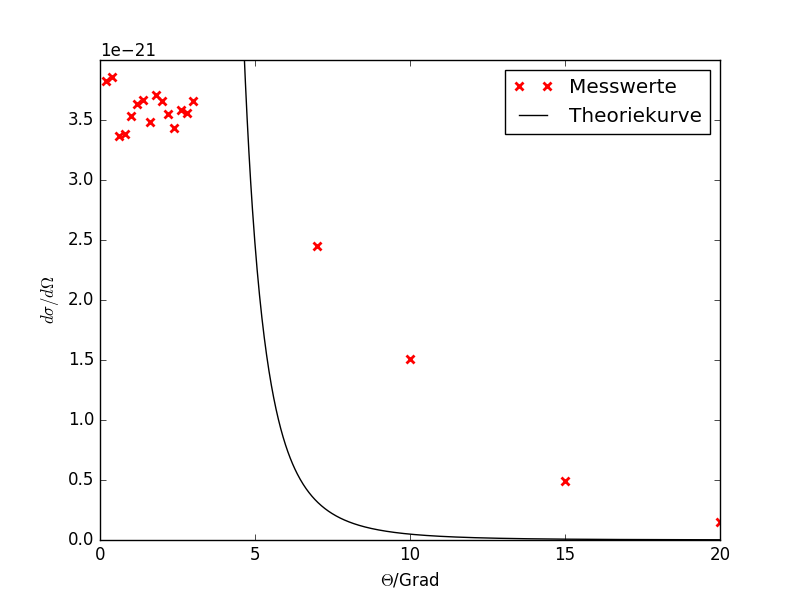
\includegraphics[width=15cm]{skripte/ruther.png}
    \caption{Messwerte und Theoriekurve f"ur das Rutherford-Streugesetz bei der $\SI{2}{\micro \meter}$-Goldfolie.}
    \label{plot:ruther}
  \end{figure}

  Wie zu erkennen ist, zeigen die Messwerte neben dem insgesamt abfallendem Trend keine gute "Ubereinstimmung mit der Theoriekurve.

  \newpage



  \subsection{Nachweis von Mehrfachstreuungen und und $Z$-Abh"angigkeit der Rutherford-Streuformel}



Die Messwerte für die Folien aus verschiedenen Materialien sind in Tabelle \ref{tab:werte} aufgelistet.

\begin{table}[H] 
\centering
\begin{tabular}{c|c c c c c c c}

	Folienmaterial & Foliendicke & Z & N [$\cdot 10^{28} \frac{1}{m^3}$]& Zeit t [s]& Zählrate n & n/t [s$^{-1}$] & $log(\frac{I_\alpha}{Nx})$ \\ 
	\hline 
	Aluminium & 3 $\mu$m & 13 & 6,022 & 120  & 619 & 5,15 & -22,545 \\ 

	Bismut &1 $\mu$m & 83 & 2,818 & 120 & 705 & 5,87 & -21,681\\ 

	Gold & 2 $\mu$m& 79 &  5.910 & 120 & 121 & 1,008 & -23,069\\ 

\end{tabular} 
	\caption{Messwerte für Folien aus unterschiedlichem Material} 
	\label{tab:werte}
\end{table}
 

\begin{figure}[H]
	\centering
	\includegraphics[width=12cm,height=8cm]{auswertung/v16_plot2.pdf}
	\caption{Z-Abhängigkeit}
	\label{img:grafik-dummy}
\end{figure}

Um die Z-Abhängigkeit zu bestimmen wird der Logarithmus von $\frac{I_\alpha}{Nx}$ gegen den Logarithmus von Z aufgetragen und eine Ausgleichsfunktion die durch $f(x)=a\cdot x+b$ gegeben ist an die Messwerte angepasst. \\
Aus der Ausgleichsrechnung ergeben sich für die Parameter a und b

\begin{align*}
a= 0,25 \pm 1,51 
\\
b= -22,84 \pm 2,54 
\end{align*}

a ist in dem Fall die Potenz der Z-Abhängigkeit. Das lässt drauf schließen, dass die Streuung von der Bethe-Bloch Formel beschrieben wird.


